\section{Comparison Matrix}\label{sec:matrix}

% ANTOINE -> TODO

% TODO - From reviewer 1 : Section 4.1: The section present a way to select papers, but it is not clear how to select papers concretely. The last three paragraphs in Section 4.1 should be expanded.

In this paper, we propose a fine grain analysis of the API functionality level and a set of comparison matrix to assist the architect in his task of selecting the right technology to build his system. 
Today, there is no single technology to manage all the requested features. Among available technologies, we distinguished three categories:

\begin{itemize}
    \item Interface Description Language (IDL): provide a vocabulary to document domain, functional and non-functional aspects of the API;
    \item Data-Interchange Formats: provide a data-structure, a vocabulary and a layout to share a textual representation of a resource to a user, including its meta-data such as profiles and semantic;
    \item Implementation Frameworks: guide developers in the implementation of the system.
\end{itemize}

In this section we present one comparison matrix per category. Each matrix classifies technologies along the eight levels of the WS3 maturity model, and a fourth category called "other" that contains extra criteria to highlight differences between listed technologies which are not included in the WS3 maturity model. As we showed in the previous section, the WS3 classification is too coarse-grained to grasp all important differences between systems of the same maturity level. Therefore, we present a set of precise criteria for each level to highlight these differences.

\subsection{Comparison Matrix Design Methodology}

% TODO - From reviewer 2 : My impression is that the paper only accounts the result of the web search, and developers' expertise is not actually leveraged. Which are the daily problems developers face? Go deeper with their experience. The framework is intended to be used by developers, you should take into account their insights from the trenches. Interview people from your company if needed, and provide links to their responses/questionnaires.

% TODO - From reviewer 2 : In the same direction, shouldn't popularity be a possible, cross-cutting criteria for comparison? if I choose technology X I'd expect to have a vibrant community to help me with any problem that may arise.

% TODO - From reviewer 2 : The methodology steps can be shortened, as they do not add any useful information. How did you verified the criteria (step v) w.r.t. your previous projects? Provide an example.

% TODO - From reviewer 2 : I cannot stand the number of acronyms the paper introduces. I acknowledge that it's difficult to present big names on tables but this is impossible to follow. E.g., You could numerate or codify approaches (most of them already have a short name) and put them as columns (criteria as rows).

The design of the comparison matrix follows a 5 steps sequential process: (i) looking for candidate technologies, (ii) selecting candidate technology, (iii) deep reading and understanding of each candidate technology, (iv) elaboration of fine grain criteria to characterized and differentiate technologies, (v) verification that the elaborated criteria suited all technologies and the need from XXX developers, and finally (vi) verification that the elaborated criteria highlighted the differences between technologies.

The research of candidate technology (step i) was done through the following steps:

\begin{enumerate}
    \item Identification of the technologies to document APIs. Methods: (i) searching Google and Google Scholar for "service description", "web service description", "web API description", "semantic web service description", "interface description language", "restful service description", "rest API documentation", "rest modeling", "web service modeling" (ii) searching for tools automating tasks from services description, using keywords: "matchmakers", "service composition", "service discovery", "rest service analysis" and (iii) reading the thesis Third Generation Web APIs \cite{lanthalerthird} and \cite{scherer2016description}.
    %Lanthaler:2013:CGW:2487788.2487799
    \item Identification of the technologies to exchange textual documents representing data across distributed systems. Method: (i) searching Google and Google Scholar for: "hypermedia document", "hypermedia format", "RDF format", "RDF document", "data-interchange format", "hypermedia media-type", "semantic web media-type".
    \item Identification of the technologies to implement web APIs. Method: searching Google and Google Scholar for "hateoas framework", "hypermedia framework", "semantic restful framework", "semantic web framework", "linked data framework", "rest API framework", "restful service framework".
    \item Identification of tools to ease the selection of a features set for Web APIs. Method: searching Google and Google Scholar for "rest api best practices", "richardson maturity model", "semantic rest maturity model", "hypermedia api maturity model", "web api best practices", "web api/services categorization".
    \item Selecting papers related to building and evaluating Web APIs from the proceedings of the International Conference on Web Engineering and WS-REST.
\end{enumerate}

From these researches, we selected papers (step ii), articles and web pages that were either the description of a technology, a comparison of technologies or a tool leveraging these technologies. We opened our research to technologies from the 1990s to today. 
From the selected papers and articles, we listed the IDLs, data-interchange formats and frameworks still available to use today.
Then, we read the specification of each chosen technology (step iii) and elaborate classification criteria (step iv). All the raw material used to elaborate this classification is available online\footnote{\url{https://anonymous.4open.science/repository/14273e30-d332-446a-b5a0-df91239532ab/}}. 

We then verified (step v) that the classification criteria suited the needs we had on previous projects we made at  XXX\footnote{company name has been removed for double blind review process} for large companies. 

As a final step (step vi), we read the specifications again to validate that the selected criteria highlighted differences and commonalities well, and to verify results.

All criteria are listed in table \ref{criteria}. Only machine-processable descriptions are considered.

\begin{table*}[ht]
\begin{tabular}{ |P{1.5cm}|p{8cm}| } 
 \hline
 \multicolumn{2}{|c|}{\textbf{Design > Resources}} \\
 \hline
 \textbf{MT} & Models/consider available media types \\
 \textbf{MR} & Models resources \\
 \textbf{MRA} & Models resources' attributes \\
 \textbf{SC} & Separates domain model from URI model \\
 \textbf{OTO} & Operations are associated to their own input and output data model \\
 \hline
 \multicolumn{2}{|c|}{\textbf{Design > Protocol Compliance}} \\
 \hline
 \textbf{MRO} & Supports association of HTTP Verbs to operations \\
 \textbf{EXT} & Extensible with custom data-interchange formats \\
 \textbf{CN} & Support content-negotiation \\
 \hline
 \multicolumn{2}{|c|}{\textbf{Design > Atomic Resources}} \\
 \hline
 \textbf{EAR} & Enforces that the full resource is the smallest data-set operations can handle \\
 \hline
 \multicolumn{2}{|c|}{\textbf{Profile > Interaction}} \\
 \hline
 \textbf{DR} & Describes resources' properties \\
 \textbf{OSD} & Describes HTTP operations \\
 \textbf{LT} & Describes templated URIs \\
 \textbf{CR} & Describes available interchange formats for Read Requests \\
 \textbf{CU} & Describes available interchange formats Update Requests \\
 \textbf{CM} & Describes HTTP verb associated to an operation \\
 \textbf{RUN} & Targets runtime information-enriched description \\
 \textbf{PS} & Supports pagination description \\
 \hline
 \multicolumn{2}{|c|}{\textbf{Profile > Domain}} \\
 \hline
 \textbf{HL} & Provides hyperlinks to other resources as meta-data \\
 \textbf{HYP} & Hypermedia controls \\
 \textbf{MC} & Models and describes business constraints on the data model \\
 \textbf{TI} & Support type inheritance \\
 \textbf{LNM} & Links are modeled by the framework, not added manually in request handlers \\
 \textbf{COA} & Describe conditions to denote an operation/link availability, otherwise the model says they are always available \\
 \textbf{CC} & Conditions for operation/link availability use more information than current resource state, such as the application context, or user-provided information \\
 \textbf{AUT} & Model the authentication mechanism \\
 \textbf{RS} & Describe resources' states \\
 \textbf{SLA} & Describe non-functional properties such as Service Level Agreement \\
 \textbf{ERR} & Describe errors \\
 \hline
 \multicolumn{2}{|c|}{\textbf{Semantic > Description}} \\
 \hline
 \textbf{SD} & Semantically describes resources' properties and HTTP operations \\
 \textbf{DC (opt.)} & Support machine-interpretable and deterministic conditions to denote an operation/link availability \\
 \textbf{RDF} & Support the addition of other RDF vocabularies - makes it RDF-compatible \\
 \hline
 \multicolumn{2}{|c|}{\textbf{Semantic > Linked Data}} \\
 \hline
 \textbf{CL} & Support giving human-interpretable semantic meaning to links \\
 \textbf{SCL} & Support giving semantic meaning to links from RDF vocabulary \\
 \hline
 \multicolumn{2}{|c|}{\textbf{Others}} \\
 \hline
 \textbf{JSON} & JSON-based format \\
 \textbf{ECD} & Entity-centric document as opposed to triple-centric \\
 \textbf{NOM} & No modification on the structure compared to an original JSON file, limited to adding more information \\
 \textbf{HF} & Made for human-readability \\
 \textbf{MF} & Made for machine-readability \\
 \textbf{CUR} & Support for Curies \\
 \textbf{PX} & Uses prefix for reserved keywords to avoid name collision \\
 \textbf{SML} & Support several meta-data level \\
 \textbf{ERS} & Transfer the resource's state explicitly \\
 \textbf{TAR} & Operations have a field to indicate which URI the operation targets, allowing to reference them as resources \\
 \textbf{FSM} & Model the system as a FSM \\
 \textbf{RS} & Model resources as FSM, not only the system \\
 \textbf{STA} & Targets static documentation \\
 \textbf{INC} & Documentation can be split into several pieces \\
 \textbf{FF} & File Format \\
 \textbf{PL} & Programming Language \\
 \textbf{LGEN} & Links to other resources hold by the system are generated at runtime, not written as code \\
 \hline
\end{tabular}
\caption{Matrix Comparison Criteria}
\label{criteria}
\end{table*}

\subsection{Interface Description Language}

% TODO - From reviewer 2 : It's impossible to cover all approaches but you should consider including LRA (Linked Rest APIs) - Linked REST APIs: A Middleware for Semantic REST API Integration, D Serrano, E Stroulia, D Lau, T Ng, Web Services (ICWS), 2017 IEEE International Conference on, 138-145
% and check its related work for others.

% TODO - from reviewer 2 : Include a column on the figures summarizing the number of criteria met by each approach.

% TODO - from reviewer 2 : How did you get columns that are not covered by at least one approach? From the protocol (sec 4.1) it seems that you extracted the criteria by analyzing existing technologies, this means, at least one technology offered it.

Interface Description Languages (IDLs) provide a vocabulary to document domain, functional and non-functional aspects of the API. Non-RDF IDLs are tied to a fixed set of file formats. Meta-models describing Web APIs are IDLs not tied to a file format. We also consider meta-models in this section. We identified 16 candidates that are classified according to 32 criteria in Figure \ref{idl-matrix}.

When IDLs and data-interchange formats are both compatible with RDF, they can be combined to form a file format that can be used as both the data-interchange format and the IDL. This has great benefits in terms of complexity and maintainability.

\subsubsection{Proper Meta-Models}

Among the 16 classified IDLs, 4 are meta-models. In \cite{Rapido} authors present a tool to sketch CRUD or Hypermedia APIs. When selecting Hypermedia APIs, users have to choose one media-type, either HAL or Collection+JSON and then start sketching the application using state machines. \cite{Schreier:2011:MRA:1967428.1967434} models each resource type as a finite state machine with deterministic state transitions. In this model, each resource type has a single initial state, operations can go beyond CRUD and conditions can be modeled to inform the availability of operations. However, conditions are not modeled in more details, which does not make them machine-interpretable. Authors propose to add this capability in future work. In \cite{10.1007/978-3-642-22233-7_24}, authors propose to model the whole system as a non-deterministic state machine. This method makes software agents unable to discover the set of messages to exchange in order to make available an operation that is not at the moment the user would like to invoke it. Haupt et al. \cite{10.1109/ICWS.2014.30} propose a very thorough multi-layered model that separates the domain model from the URI model. It does not allow specifying conditions on the availability of operations and see resources as having a static structure, making it impossible to represent different state of a resource with different classes. 

\subsubsection{Meta-Models from Interface Description Languages}

The 11 interface description languages we found are Hydra Core Vocabulary \cite{Lanthaler:2013:CGW:2487788.2487799}, Atom Syndication Format\cite{AtomSF}, WSDL+SAWSDL, WADL, OpenApi (used by Swagger), API Blueprint, hREST + microWSMO, RESTdesc, RADL, RAML and I/O Docs. We decided to include WSDL+SAWSDL even though it targets RPC-like applications over HTTP \cite{john2012framework}, because it tackles the problem of semantically describing HTTP services.

% FIGURE OF THE IDL CLASSIFICATION
\begin{figure*}[t]
\caption{Interface Description Languages Comparison Matrix}
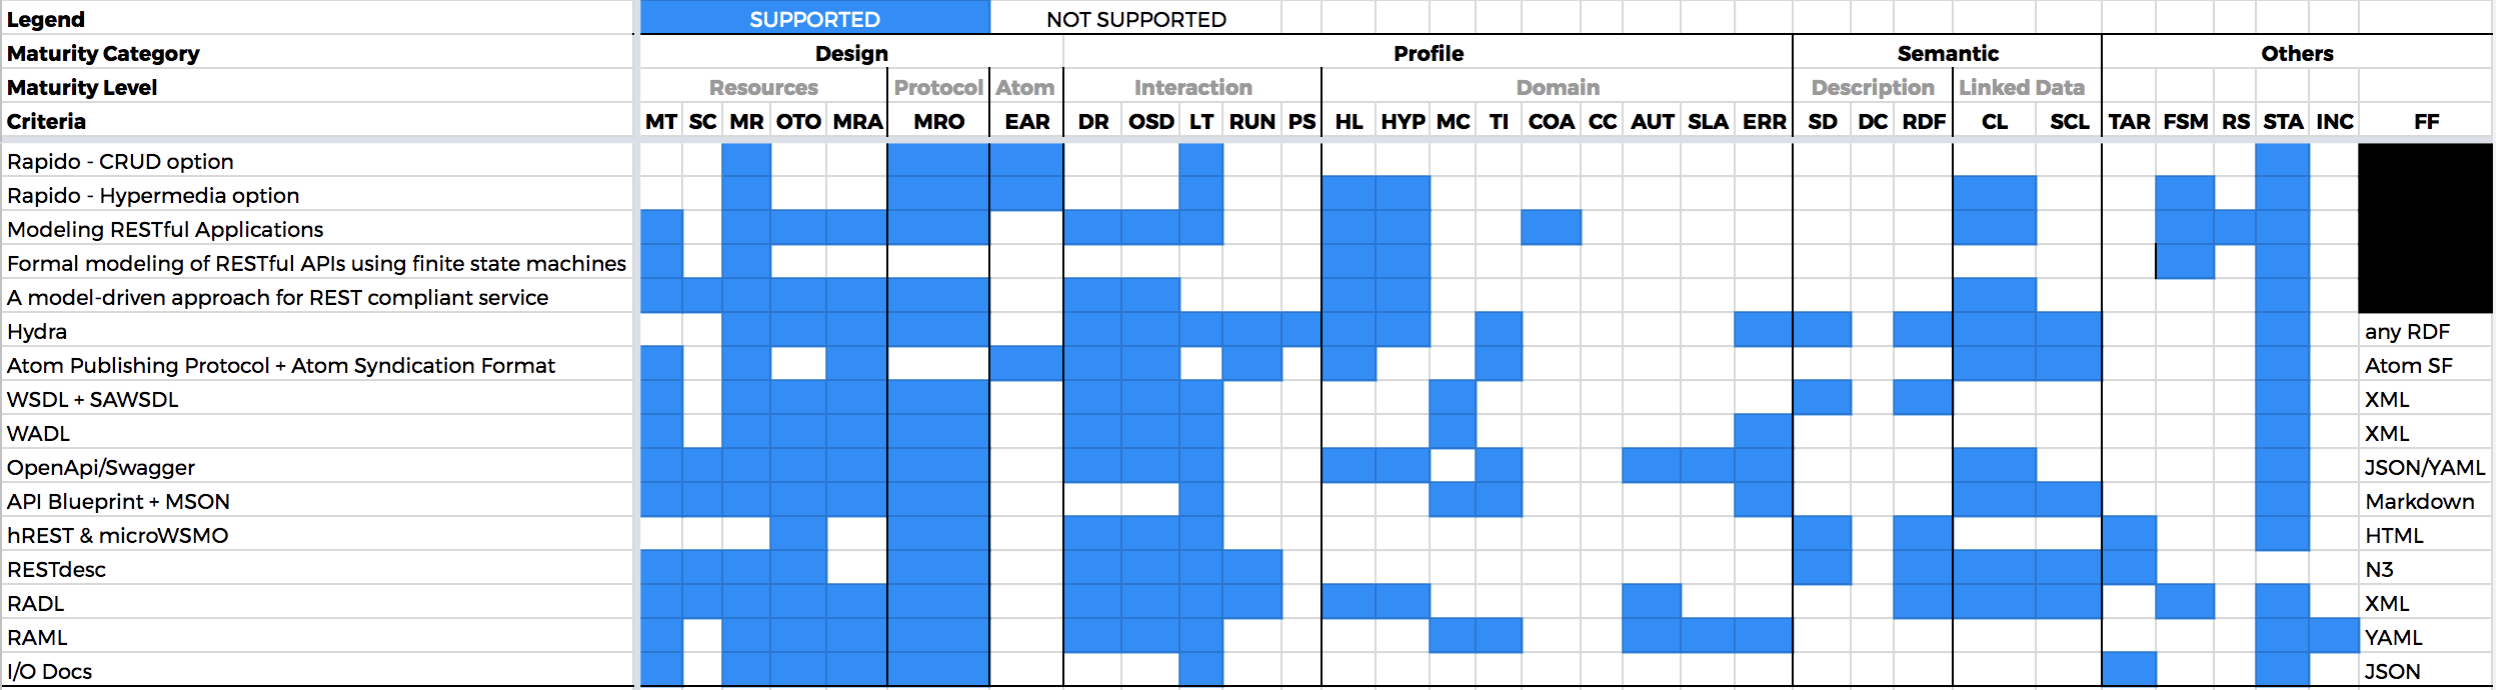
\includegraphics[width=1\textwidth]{figures/IDL.png}
\label{idl-matrix}
\end{figure*}

\subsubsection{Conclusions}

The first thing the matrix highlights is that most IDLs ignore the domain and semantic description of APIs. In addition, they focus on the static documentation of the entire API made for developers, rather than the documentation enriched with information on the current state of the system to guide users when browsing the API.

From this matrix, we observe that Hydra and RESTdesc are the two approaches reaching the highest maturity level. This is because they both semantically describe metadata, use additional RDF vocabularies and target API documentation enriched with execution information.

Only one approach \cite{Schreier:2011:MRA:1967428.1967434} support conditional availability of links between resources and no one makes this meta-data machine-interpretable. This makes software agents unable to find a way to make an operation available when it is not.

Four technologies support the addition of business constraints to the model, and three are machine-processable. We encourage authors of meta-models to add this feature to their technology because it is a step forward in lowering coupling and improving user experience. For example, this allows forms to be automatically generated with client-side data validation.

Finally, this matrix highlights that three out of four scientific publications recommend the modeling of RESTful systems as state machines whereas all except one IDL authors ignore this technique. However, the use of deterministic state machines encourages API designers to think about the domain model in depth. It is then easier to determine if an operation on a resource is not available.

\subsection{Data-interchange formats}

The data-interchange formats can be differentiated based on their compatibility with RDF, which determines if they are extensible. Because they are extensible, RDF formats propose very few features by default. We selected three vocabularies (i) Hydra, (ii) HTTP RDF and (iii) SHACL, an RDF schema validation vocabulary, that we combined with one RDF format, JSON-LD, to show what is possible to do.

When building an API that provides no meta-data, JSON, XML and YAML are the three formats widely used in industry.

On the other side, when the system to build have to send meta-data, no data-interchange formats is considered as a standard today. We found eleven propositions on the web, from scientific publications, GitHub repositories, private web sites, IETF and W3C drafts. They are classified in Fig. \ref{interchange-formats-matrix} according to 26 criteria.

% FIGURE OF THE INTERCHANGE FORMATS CLASSIFICATION
\begin{figure*}[t]
\caption{Data-interchange Formats Comparison Matrix}
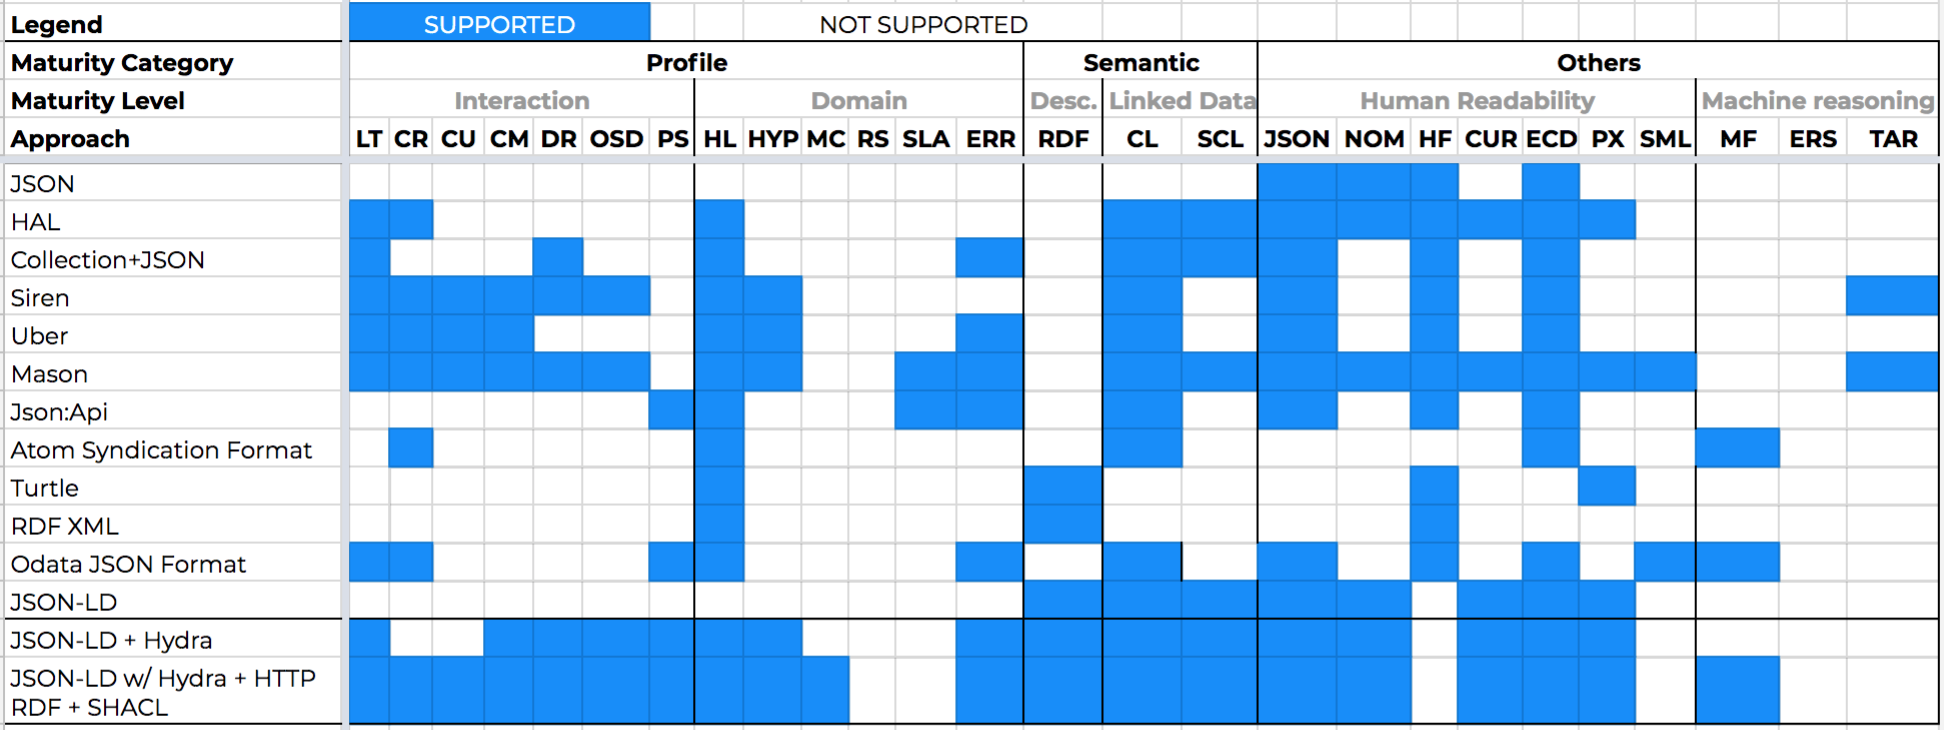
\includegraphics[width=1\textwidth]{figures/DIF.png}
\label{interchange-formats-matrix}
\end{figure*}

\subsubsection*{Conclusions}

On the one hand, non-RDF formats do not allow to reach any level on the semantic axis. However, some of them allow to link the data to others, and to reach the highest level on the \textit{Profile} dimension.
On the other hand, RDF formats can become very expressive when combined with vocabularies. The example with JSON-LD + Hydra + HTTP RDF + SCHACL shows this. However, they require more effort to find appropriate vocabularies on the web.
Furthermore, the matrix highlights that most formats are not readable by machine.

Last, the matrix shows that no format support the description of constraints on the data neither the advertisement of resource's state. Though, most scientific approaches we found describe REST APIs as state machines. Providing the resource's state would ease machine-reasoning. On the other hand, describing the constraints could greatly decrease coupling and increase user experience.

\subsection{Implementation Frameworks}

% TODO - from reviewer 2 : Maybe it's out of scope but I think Loopback (https://loopback.io/) should be analyzed as a framework as it provides/leverages some semantic sugar.

Implementation frameworks are software libraries that guide developers through the implementation of Web APIs. We limit the comparison to frameworks that claim to support HATEOAS. We identified six frameworks that do so.

In \cite{salvadori2014framework} authors propose a Java framework based on JAX-RS 2.0 that uses annotations to semantically describe REST APIs. The end result is a JSON-LD document, enriched with the Hydra vocabulary, that describes the whole API. In \cite{parastatidis2010role} Parastatidis et al. present Restfulie, a framework to ease the development of REST APIs using resources, content-negotiation and state transitions as its core building blocks. Besides these frameworks, we found that API-Platform, Spring HATEOAS, JAX-RS and Ripozo support HATEOAS features. They are classified in Fig. \ref{frameworks-matrix} according to 29 criteria.

% FIGURE OF THE INTERCHANGE FORMATS CLASSIFICATION
\begin{figure*}[t]
\caption{Implementation Frameworks Comparison Matrix}
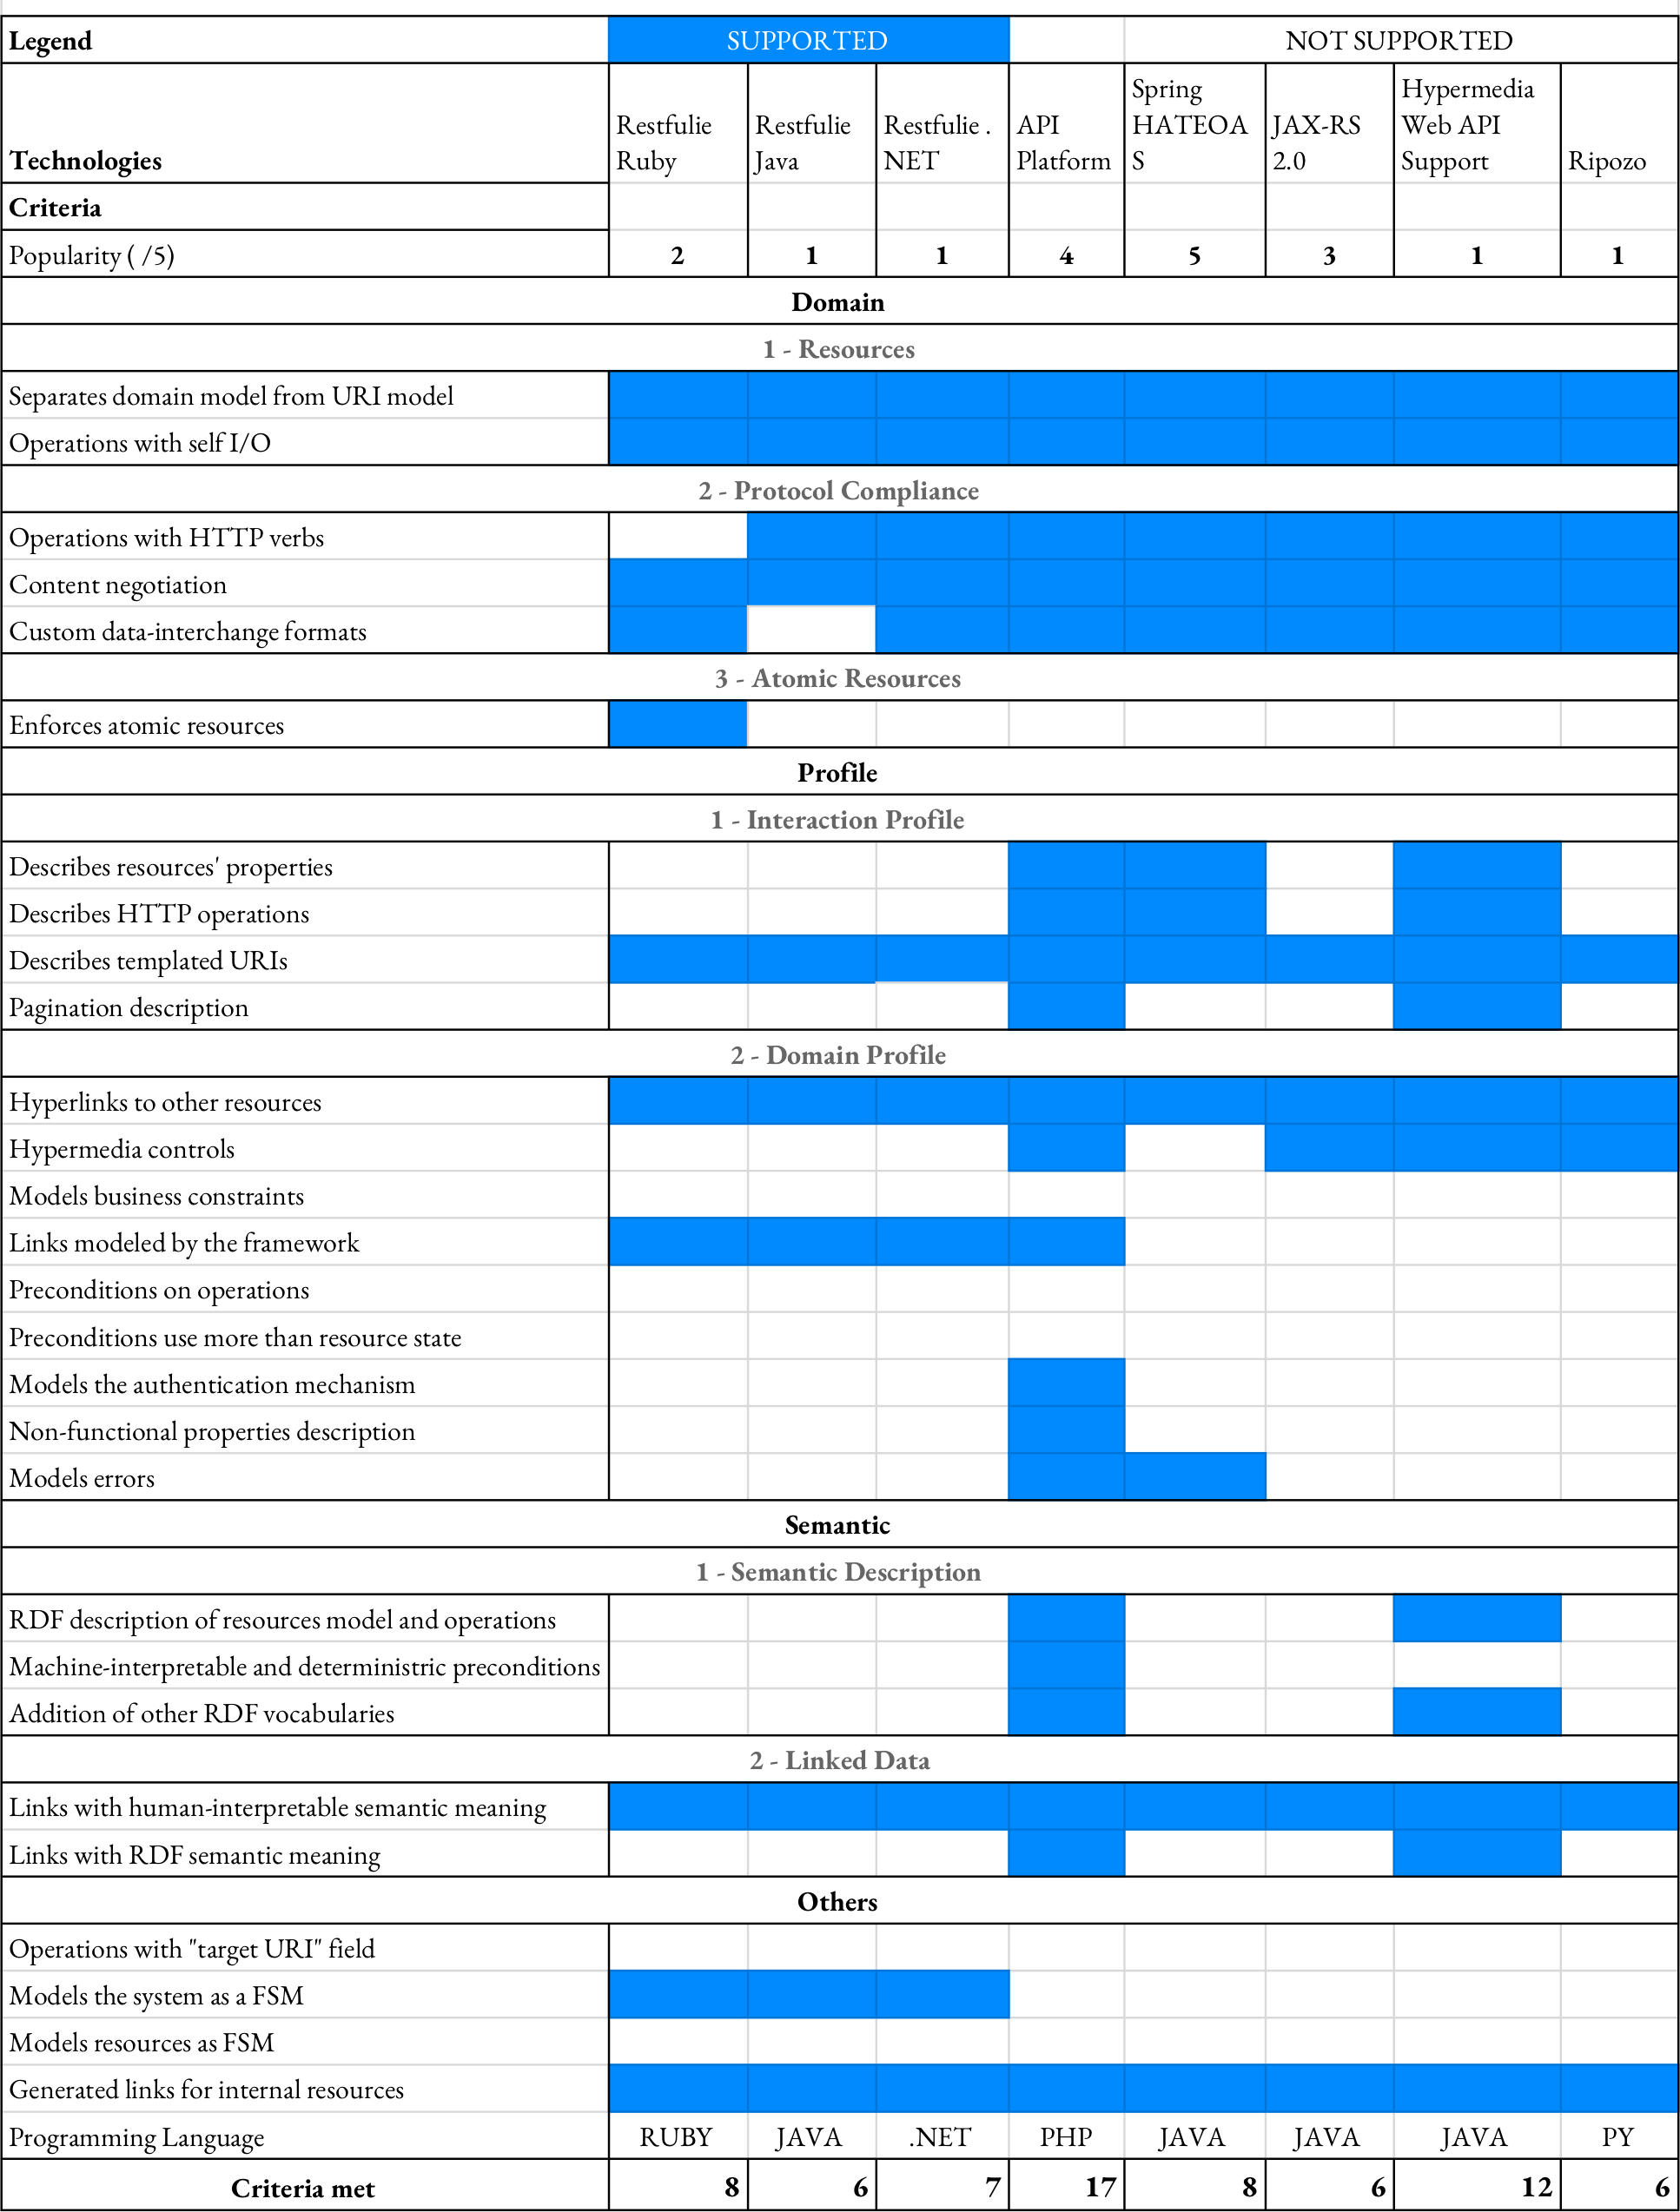
\includegraphics[width=1\textwidth]{figures/frameworks.png}
\label{frameworks-matrix}
\end{figure*}

\subsubsection*{Conclusions}

Despite the fact that only one framework enforces the atomic resources constraint, all frameworks allow to reach the highest level of maturity on the Design axis easily. This is because supporting the Atomic feature is a constraint that can be easily added by the developers themselves. 

We notice that only \textit{APIPlatform} and \textit{Restfulie} support a mechanism to model links instead of adding them programmatically in the resource, thus increasing maintainability.

Otherwise, most framework do not ease the process of documenting and making the API Semantic Web and Linked Data compatible. To us, this is the biggest challenge framework designers are facing today.

As with IDLs, most creators of frameworks do not provide mechanisms to describe resources as state machines even though it could bring the same benefits.
